%  A simple AAU report template.
%  2015-05-08 v. 1.2.0
%  Copyright 2010-2015 by Jesper Kjær Nielsen <jkn@es.aau.dk>
%
%  This is free software: you can redistribute it and/or modify
%  it under the terms of the GNU General Public License as published by
%  the Free Software Foundation, either version 3 of the License, or
%  (at your option) any later version.
%
%  This is distributed in the hope that it will be useful,
%  but WITHOUT ANY WARRANTY; without even the implied warranty of
%  MERCHANTABILITY or FITNESS FOR A PARTICULAR PURPOSE.  See the
%  GNU General Public License for more details.
%
%  You can find the GNU General Public License at <http://www.gnu.org/licenses/>.
%
\input{setup/preamble.tex}% package inclusion and set up of the document
\input{setup/hyphenations.tex}% 
\input{setup/macros.tex}% my new macros


\begin{document}
\begin{titlepage}



\begin{center}
\newcommand{\HRule}{\rule{\linewidth}{0.5mm}}
\HRule \\[0.4cm]
\Huge Software Innovation Eksamen \\[0.3cm]
	\Large Grupperne SW807 og SW808\\[0.4cm]

\HRule \\[1cm]
\noindent
\begin{minipage}{7cm}
  \textbf{SW807:}\\
  {\small Mikael Elkiær Christensen\\
  Mikkel Sandø Larsen\\
  Stefan Marstrand Getreuer Micheelsen\\
  Bruno Thalmann}
\end{minipage}
 \hfill
\begin{minipage}{5cm}
  \textbf{SW807:}\\
  {\small Søren Skibsted Als\\
  Lars Andersen\\
  Lasse Vang Gravesen\\
  Mathias Winde Pedersen}
\end{minipage}

\vfill
{\Large Software Innovation}
\\ ~\\
{\large Software 8. Semester, Aalborg Universitet, Foråret 2015}

\end{center}
\end{titlepage}

\pagestyle{empty} %disable headers and footers
\pagenumbering{roman} %use roman page numbering in the frontmatter
%\input{frontpage.tex}

\pagestyle{fancy} %enable headers and footers again
\setcounter{tocdepth}{1}
\listoftodos
%\input{sections/preface.tex}
%mainmatter
\pagenumbering{arabic} %use arabic page numbering in the mainmatter

\section{Relationen mellem projekt og de fire varianter}
%A relation of your project to software innovation variants (see Essence-book Section 5.1).
Dette afsnit beskriver mulige syn på software innovation i lyset af de fire forskellige varianter heraf\citet[Afsnit 5.1, Side 30-31]{art:essence}.
Afsnittet beskriver herved fire forskellige tilgange til software innovation i kontekst af PsyLog projektet.

\subsection{Produkt innovation}
% Product innovation is about developing new or improved software-intensive products

\subsection{Proces innovation}
% Process Innovation is about developing software-intensive solutions that offer users new or improved ways to produce their existing products or services

\subsection{Projekt innovation}
% Project innovation is when existing software solutions are fitted into new application domains (illustrated in Section 4.3) – what Tidd et al. labels position innovation.

\subsection{Paradigme innovation}
% Finally, Paradigm innovation is when software-intensive solutions are coupled with changes in the ‘mental models’ which frame what an organization is about; who the users are; or what the market is or wants (illustrated in Section 4.1).

\section{VBM review}
For at give et eksempel på et VBM review beskrives vores vision inquiry review.
Vores vision inquiry baserer sig på teorien beskrevet i \citet[afsnit 10.5, side 66]{art:essence}.
At foretage dette review sikrer at visionen giver en beskrivelse af relationen mellem problem og løsning der er rammende.
Dermed ikke sagt at visionen skal give en udtømmende beskrivelse, men rettere at give en forståelse af hvad hovedidéerne er ved projektet.

Visionen der foretages et Vision Inquiry på er fra konfigurationstabellen der kan ses i \cref{tab:konfigurationsTabel}.
Vision Inquiry   F-16
\begin{description}[style=nextline]
	\item[Is the Vision brief and communicable?]
		Visionen om F-16 er kortfattet. 
		Dog kan der herske forvirring da man kan forestille sig død og ødelæggelse i stedet for modularitet der menes.
		Dog understøttes denne vision af andre metaforer og en proposition, hvorfor dette ikke regnes for et problem.
	\item[Does the Vision aptly link solution to problem?]
		Visionen passer godt på løsningen, da løsningen er modulær ligesom F-16 flyet.
	\item[Are the Grounds related to the Use context?]
		Nej, de er ikke relaterede da use context snakker om teknologi hvor Grounds snakker om affektive lidelser.
	    Der mangler altså et bindeled mellem hvad teknologien har med affektive lidelser at gøre.
	    En mulig omformulering kunne være at omformulere grounds til "depressions- og mani-perioder opdages for sent, men kan opdages vha. data fra smartphones".
	\item[Does the Warrant provide good reason to solve the problem?]
		Ja, det er en meget god grund til at løse problemet.
	\item[Does the Qualifier identify key limitations relative to the Challenge?]
		Den siger man skal have en basal viden om smartphones.
		Begrænsning i forhold til teori om registrering af adfærdsændringer nævnes ikke.
	\item[Does the Rebuttal recognize the solution as acceptable?]
		Ja, det er meget god grund, da man kan reducere antallet af behandlinger, og dermed omkostninger på dette felt.
	\item[Does the features offer a sound idea about how the solution solves the problem?]
		Features giver ikke en særlig god ide om hvordan de løser problemet.
		Savner bedre beskrivelse af interne features.
\end{description}

Findings fundet er derefter input til den næste sprint planning aktivitet, og dette kan også føre til ændringer i visionen. 

\chapter{Essence}
I dette afsnit bliver diverse Essence emner præsenteret og detaljeret.
\section{Beskrivelse af problem}
Der er valgt at arbejde med vores semesterprojekt som omhandler en mobil app der kan assistere patienter med psykiske lidelser.

Den nuværende praksis kræver at patienten bliver diagnosticeret af en psykolog.
Projektet forsøger at supplere med en metode, der kan aflaste psykologen og assistere patienten i sin hverdag.

Dette skal gøres ved hjælp af en mobil platform der udnytter de sensorer der er på en smartphone.
Disse sensorer kan bruges til at opsamle information om patientens adfærd uden at forstyrre patienten.
Ydermere kan en smartphone interagere med patienten i løbet af dagen. 
Den opsamlede data kan derefter analyseres for at forsøge at give et billede af patientens stemningsleje.

Projektet søger at udvikle en platform, der udgør et fundament for moduler der kan assistere patienter med affektive lidelser, på en mobil platform, således at man kan supplere den nuværende behandling hos en læge.
%\begin{figure}
\includegraphics[scale = 0.65,trim = 1cm 3cm 6cm 2cm, angle = 90, clip]{tidlig_konfigurationstabel}
\caption{Den tidlige konfigurationstabel.}
\label{tidlig_konfigurationstabel}
\end{figure}

%\section{Tidlig konfigurationstabel}
\bruno{tilpas}
% Systematisk beskrivelse af konfigurations tabel.
\section{Konfigurationstabel}
En konfiguration af et system er en kombination af elementer, og en konfigurationstabel beskriver den konfiguration.

Denne beskrivelse er baseret på \citet[Afsnit 3.2, Side 16-21]{art:essence}.

Den øverste række i \cref{tab:konfigurationsTabel} navngiver de fire Views i Essence: Paradigm, Product, Project og Process.

`Focus' rækken repræsenterer de største problemer og løsninger i projektet. 
Udfordringen er tiltænkt til at være om man kan bruge en mobil til at overvåge adfærd af unipolare og bipolare patienter og gøre dem opmærksom på adfærdsændringer og dette er så tiltænkt at disse patienter åbner en applikation på denne mobil hvor de vil blive blive givet et overblik og derved få at vide om der har været adfærdsændringer. 
Det er så vigtigt at systemet skal kun observere og informere.
Løsnings strategien er så at bruge en smartphone, og udvikle et system som kan registrere data fra forskellige sensor moduler og gemme det på telefonen som den bliver brugt af patienten.
Data den indsamler skal være objektiv og spore patientens sindstilstand såsom en fitness tracker sporer fysisk tilstand samt at systemet skal være ekspandérbart, så vision for systemet er så at den skal fungere som en fitness tracker, en objektiv dagbog og et F-16 fly.
Denne data kan så bruges til analyse og blive undersøgt om der er nogle ændringer i patientens opførsel og skal let kunne aflæses af patienten hvorfra de kan få relevant information fra den præsenterede data. 

`Overview' rækken repræsenterer projektets stakeholders. Hoved perspektivet er selvfølgelig fra patienterne, da det er dem som skal bruge produktet men der er også sponsorer som er interesseret i at se projektet være en succes da det vil gøre at deres patienter vil få det nemmere. 
Designet på projektet er simpelt idet der bruges mobil eller wearables til sensor input og at denne data gemmes og analyseres på mobilen, og at det skal udvikles på Android.
Argumentet for at lave et sådant projekt er, at depression og mani ofte opdages for sent, hvilket i det fleste tilfælde gør situationen værre.
Hvis symptomerne identificeres så perioden opdages tidligt kan den måske forhindres, hvilket kan spare staten en del udgifter til behandlinger og indlæggelser.
Der er dog det problem at en smartphone baseret løsning som der her sigtes efter selvfølgelig kræver en smartphone, og også stiller lidt krav til at folk kan bruge deres smartphone.
Dette er dog bare et minimalt problem da en stor del at befolkningen har smartphone nu om dage så derfor kan man også gå ud fra de kan finde ud af at bruge den på et acceptabelt niveau.
Selv hvis en potentiel bruger ikke har en smartphone, koster den lettilgængelige teknologi ikke så meget, så at investere i den som et behandlingsmiddel er en reel mulighed.
For at evaluere systemet kan der bruges et fokusgruppemøde og integrationstest for at sikre det er modulær, fleksibel, kombinerbar og kommunikativ.

`Details' rækken repræsenterer nøgle scenarier, nøgle komponenter og features.
Desuden indeholder det sidste felt i denne række også findings.
Findings er speciel da den bruges som et input til den næste Sprint Planning aktivitet, se \citet[Afsnit 8.5, Side 54]{art:essence}. 
Findings kommer som et resultat af evaluering af systemet. 
Disse findings er at der er problemer med højt pladsforbrug og at systemet har mulige sikkerhedsproblemer. 

\begin{figure}
\includegraphics[scale = 0.65,trim = 1cm 3cm 6cm 2cm, angle = 90, clip]{KonfigurationTabel-frarapport.pdf}
\caption{En konfigurationstabel af systemet.}
\label{tab:konfigurationsTabel}
\end{figure}

% Systematisk beskrivelse af konfigurations tabel.
\section{Konfigurationstabel}
En konfiguration af et system er en kombination af elementer, og en konfigurationstabel beskriver den konfiguration.

Denne beskrivelse er baseret på \citet[Afsnit 3.2, Side 16-21]{art:essence}.

Den øverste række i \cref{tab:konfigurationsTabel} navngiver de fire Views i Essence: Paradigm, Product, Project og Process.

`Focus' rækken repræsenterer de største problemer og løsninger i projektet. 
Udfordringen er tiltænkt til at være om man kan bruge en mobil til at overvåge adfærd af unipolare og bipolare patienter og gøre dem opmærksom på adfærdsændringer og dette er så tiltænkt at disse patienter åbner en applikation på denne mobil hvor de vil blive blive givet et overblik og derved få at vide om der har været adfærdsændringer. 
Det er så vigtigt at systemet skal kun observere og informere.
Løsnings strategien er så at bruge en smartphone, og udvikle et system som kan registrere data fra forskellige sensor moduler og gemme det på telefonen som den bliver brugt af patienten.
Data den indsamler skal være objektiv og spore patientens sindstilstand såsom en fitness tracker sporer fysisk tilstand samt at systemet skal være ekspandérbart, så vision for systemet er så at den skal fungere som en fitness tracker, en objektiv dagbog og et F-16 fly.
Denne data kan så bruges til analyse og blive undersøgt om der er nogle ændringer i patientens opførsel og skal let kunne aflæses af patienten hvorfra de kan få relevant information fra den præsenterede data. 

`Overview' rækken repræsenterer projektets stakeholders. Hoved perspektivet er selvfølgelig fra patienterne, da det er dem som skal bruge produktet men der er også sponsorer som er interesseret i at se projektet være en succes da det vil gøre at deres patienter vil få det nemmere. 
Designet på projektet er simpelt idet der bruges mobil eller wearables til sensor input og at denne data gemmes og analyseres på mobilen, og at det skal udvikles på Android.
Argumentet for at lave et sådant projekt er, at depression og mani ofte opdages for sent, hvilket i det fleste tilfælde gør situationen værre.
Hvis symptomerne identificeres så perioden opdages tidligt kan den måske forhindres, hvilket kan spare staten en del udgifter til behandlinger og indlæggelser.
Der er dog det problem at en smartphone baseret løsning som der her sigtes efter selvfølgelig kræver en smartphone, og også stiller lidt krav til at folk kan bruge deres smartphone.
Dette er dog bare et minimalt problem da en stor del at befolkningen har smartphone nu om dage så derfor kan man også gå ud fra de kan finde ud af at bruge den på et acceptabelt niveau.
Selv hvis en potentiel bruger ikke har en smartphone, koster den lettilgængelige teknologi ikke så meget, så at investere i den som et behandlingsmiddel er en reel mulighed.
For at evaluere systemet kan der bruges et fokusgruppemøde og integrationstest for at sikre det er modulær, fleksibel, kombinerbar og kommunikativ.

`Details' rækken repræsenterer nøgle scenarier, nøgle komponenter og features.
Desuden indeholder det sidste felt i denne række også findings.
Findings er speciel da den bruges som et input til den næste Sprint Planning aktivitet, se \citet[Afsnit 8.5, Side 54]{art:essence}. 
Findings kommer som et resultat af evaluering af systemet. 
Disse findings er at der er problemer med højt pladsforbrug og at systemet har mulige sikkerhedsproblemer. 

\begin{figure}
\includegraphics[scale = 0.65,trim = 1cm 3cm 6cm 2cm, angle = 90, clip]{KonfigurationTabel-frarapport.pdf}
\caption{En konfigurationstabel af systemet.}
\label{tab:konfigurationsTabel}
\end{figure}


\section{Udløsning af Projektet}
% Essence chapter 4.
Når et projekt startes er det vigtigt at have en fælles forståelse for hvad retning man bevæger sig i.
Denne retning udspringer af det problem som udløste projektet, men kan efterfølgende ændre sig som projektet skrider fremad.

I Essence beskrives 4 typer af initierende problem; \textit{User need}, \textit{Technological opportunity}, \textit{Solution reuse} og \textit{Competitive stress}.
Disse 4 ligger op ad de 4 \textit{views} i Essence; henholdsvis \textit{Paradigm}, \textit{Product}, \textit{Project} og \textit{Process}.

Det der udløste dette projekt var en kombination af de to første; user need og technological opportunity.
Det problem at mange personer har psykiske lidelser har eksisteret i lang tid, så på denne måde er og har der været et brugerbehov, og endda et samfundsbehov, i længere tid.
Problemet ligger både i at detektere og forbygge værre tilfælde.
Yderligere bliver smartphones mere og mere udbredte, samtidig med at der opstår flere og flere krops-knyttede enheder der kan indsamle et væld af informationer om en brugers tilstand og færden.
Deri ligger problemet at udnytte den nye teknologi i forbindelse med det førnævnte problem omkring detektering og forebyggelse af psykiske lidelser.

Kombinationen af disse to initierende problemer har givet anledning til et udgangspunkt til dels i \textit{paradigm} og \textit{product} \textit{views}.
Dette har ført til et behov for en grundig analyse af problemområdet, herunder de forskellige lidelser og hvilke typer af patienter der kunne være interessante for projektet.
Samtidig har der også været fokus på produktet, i det at de mange mulige datakilder der kan tilgås gennem smartphone eller wearables har været undersøgt, samtidig med at der er udviklet en dynamisk platform der kan understøtte adskillige af disse datakilder.


\section{Vision}
\stefan{jeg tror dette afsnit skal væk, det er overlap med \ref{projectvisionrepr}}
Vores vision for projektet repræsenteres ved hjælp af Metaphor, specifikt formuleres det ved hjælp af tre metaforer.
Disse metaforer er \textit{Objektiv dagbog}, \textit{Fitness tracker} og \textit{F16 fly}.
At formulere vores vision som en metafor lader os koncist specificere hvad der er nøgleaspekterne af produktet.

Den objektive dagbog danner tanken om en dagbog baseret på objektive datakilder, hvilket svarer til sensor data, brugsdata etc.
Alt sammen data der kan indsamles uden brugerinteraktion.

Fitness trackeren som metafor planter tanken om en applikation, der løbende evaluerer ens præstationsevne, hvilket kan oversættes til mentalt helbred.

F16 fly metaforen henvender sig til platforms designet, der er tiltænkt at være en meget modulær og kraftig platform, ligesom det er tilfældet med F16 flyet hvor man kan hægte en lang række komponenter på alt efter hvad der er brug for i den pågældende situation.



\section{Use Cases}
I \citet[Afsnit 13.3, s83, nederst]{art:essence} beskrives fire forskellige elementer, der skal overvejes i forbindelse med kreationen af brugsscenarier.
Disse overvejelser skal ligge på stakeholders, kontekst, teknologi og problemer.
Stakeholders er hvem scenariet har effekt på, kontekst er i hvilke omgivelser scenariet finder sted og hvilken effekt det har, teknologi er hvilke teknologiske muligheder, der allerede eksisterer, problemer er hvad alt hvad der kunne give grundlag for en ændring.

For de scenarier der præsenteres er kontekst og stakeholders vurderet til at være de samme, selvom der i \citet[Afsnit 13.3, s83, nederst]{art:essence} siges at de sagtens kan variere fra et scenarie til et andet.

\subsection{Kontekst}
Konteksten som applikationen skal kunne bruges i er meget bred, da den omfatter hele patientens hverdag og alle tænkelige lokationer en patient kan opholde sig i løbet af sådan en dag.
Der skal derfor tages højde for at forbindelse til GPS, WIFI og mobilnetværk ikke altid er tilgængelige.
Da applikationen skal logge data om patientens færden skal der sikres håndtering af en række forskellige tilfælde angående brug og placering af smartphone.
Smartphonen kan eksempelvis være i lommen, i hånden, på et bord eller i en jakkelomme, hvor jakken hænger i entréen.
Dette betyder at konteksten kan variere fra ude i en skov uden dataforbindelse til patientens arbejde med internet adgang.

\subsection{Stakeholders}
I dette projekt er patienterne den vigtigste \textit{stakeholder}, da det er patienterne, der skal bruge systemet i hverdagen.
Systemet skal derfor udvikles på patienternes præmisser.
I dette projekt er det specifikt patienter med unipolar eller bipolar affektiv lidelse vi beskæftiger os med.

Der er et antal sponsorer tilknyttet projektet, med dette menes folk, der har interesse i projektet uden at være direkte stakeholders, da de ikke er tiltænkt at skulle bruge systemet.
Morten Aagaard har både erfaring inden for datalogi og psykologi og kan agere bindeled mellem de to discipliner.
Janne Vedel Rasmussen og Jørgen Aagaard arbejder inden for psykologifaget og kan derfor bidrage med fagrelevant information.
De har derudover en interesse i at få udviklet værktøjer, der kan bidrage til deres arbejde.

\subsection{Scenarios}\label{sec:scenario}
Her undersøges hvordan \textit{the Challenge}\bruno{Skald det være challenges eller?} bliver set fra brugerens perspektiv.
Teknikker til denne undersøgelse inkluderer at udforske systemets problemdomæne ved hjælp af \textit{Use scenarios}.

\paragraph{Use scenarios}
\textit{Use scenarios} bruges til at udforske ideer og muligheder i forhold til brugerens brug af systemet.

\subparagraph{Scenarier:}
\begin{enumerate}
	\item Patienten bevæger sig rundt i sin hverdag med smartphonen i lommen. \label{hverdag}
	\begin{itemize}
		\item Data logges i systemet, som gemmes til senere analyse.
	\end{itemize}
	
	\item Patienten vil gerne have applikationen til at fortælle hvordan den vurderer hans tilstand. \label{vurder}
	\begin{itemize}
		\item Applikationen viser at patienten udviser normal adfærd.
		\item Applikationen viser at patientens stemningsleje er lavere end normalt.
		Patienten konsulterer sin liste af lystbetonede aktiviteter og udfører en af disse.
		\item Applikationen viser at patientens stemningsleje er lavere end normalt.
		Patienten foretager sig intet og tilstanden fortsætter med at forværres.
	\end{itemize}
\end{enumerate}
Dette sidste scenarie inkluderer en kontaktperson som stakeholder.
Denne kontaktperson kan fx en patients kone, en nær ven eller en læge. 
\begin{enumerate}
	\setcounter{enumi}{2}
	\item Applikationen registrerer fald af tilstand gennem en længere periode \label{fald}
	\begin{itemize}
		\item Tilstanden rammer et kritisk niveau og kontaktperson kontaktes
	\end{itemize}
\end{enumerate}


\subsection{Problems}
I scenarie \ref{hverdag} er det et potentielt problem at smartphonen for ofte befinder sig i en kontekst hvor den indsamlede data ikke kan bruges, hvilket vil kræve en ændring.
En mulig ændring kan være i form af en måde at registrere kontekst så data kan filtreres i når det kan bruges og når det ikke kan bruges.
Et andet problem der kan opstå er, at det ser ud som om at smartphonen er på en person, men det er bare ikke patienten der benytter smartphonen.
Dette problem kræver en form for persongenkendelse så data fra andre personer kan filtreres fra.

I scenarie \ref{vurder} er det problematisk hvis patienten ikke bruger det ofte nok og derfor ikke bliver informeret om sin tilstandsændring tids nok til at det rent faktisk kan hjælpe.

I scenarie \ref{fald} kan det være et problem at bestemme det kritiske niveau ud fra individet
Desuden kan det for nogen individer kræve øjeblikkelig indlæggelse.
Hvis en sådan patient registreres i kritisk tilstand, er det ikke nok bare at kontakte en kontaktperson, men burde nok nærmere tilkalde en ambulance.
Der er også den risiko at det at kontakte en kontaktperson bliver vurderet som problematisk i forhold til patient empowerment konceptet, som projektet gerne skulle have fokus på med. \bruno{Forstår ikke den her sidste paragraf :((}
\stefan{jeg har sat en reference på, men er også lidt i tvivl om meningen med indholdet}

 %A description of use context and selected use scenarios (see Essence-book Chapter 13).
\section{Discussion of support for key use scenarios}
Ud fra disse scenarier har vi følgende tilstands klassificerings problematikker:
\begin{itemize}
\item På korrekt person?
\item Tilstands ændring?
\item Kritisk tilstand?
\end{itemize}

Den første problematik er hvordan man identificerer hvilken kontekst dataindsamlingsenheden befinder sig i, og ud fra denne vurdere hvilke datakilder der stadig bibeholder deres relevans i denne kontekst.
Eksemplet der et givet i førnævnte scenarie er at patienten har efterladt eller glemt sin telefon i sin jakke, i en sådan situation kunne man forstille sig at datakilder som for eksempel bevægelsesdata eller lydregistrering er ubrugelige.
Dog skal man også i denne sammenhæng være forsigtig, for hvis man forkaster for meget data når telefonen ikke er på en person, vil det gøre det vanskeligt at lave analyser på perioder hvor man ved at telefonen ikke holdes af en person hvilket kunne være søvn analyse. 
Det er dog ikke kun et spørgsmål om at identificere hvornår telefonen ikke er på en person.
Der skal også identificeres om det er den tiltænkte person der bærer enheden, da i disse situationer giver data der indsamles et indblik i den forkerte persons tilstand.

Den anden udfordring, at identificere brugerens tilstand, kræver indsamling af meget data fra mange forskellige kilder for at have et grundlag for en vurdering af disse.
Hvilke datakilder dette skal være kan variere meget fra individ til individ.
Et individ kunne for eksempel have brug for at få set på sit bevægelsesmønster og på sin sociale adfærd, hvor et andet kunne have brug for at få analyseret på søvn og på hvor meget han har forladt sit hjem.
At kunne se på disse er udfordrende i sig selv, da man for hver af disse skal finde ud af hvilke datakilder man har til rådighed der kan give en fornuftig information om disse, og derefter skal man finde ud af hvordan man ud fra den data kan lave en vurdering af det givne kriterie.
Når hvert kriterie er vurderet skal der laves en vurdering af tilstanden som helhed, og hvordan denne laves skal variere fra individ til individ.
Det kunne også være man valgte at inddrage brugeren i denne vurdering, enten ved at give dem spørgsmål eller ved at have dem til at gøre noget andet der kunne give et prej om hvordan de har det.

Den sidste tilstand der kan være er en kritisk tilstand, hvor det vurderes at patienten er så langt nede at der er risiko for han kan forvolde skade på sig selv eller andre.
Her er problemet hvornår man vurderer en tilstand til at være alvorligt kritisk og også hvad man rent faktisk skal gøre hvis man når frem til en sådan vurdering.
Den kritiske vurdering kunne være at man har en grundlinje for hvor lavt eller højt folks sindstilstand kan komme på en scala før den er kritisk, dog er dette nok ikke en god tilgang, da det som altid kan variere meget for hvert individ.
En anden mulighed ville være at se på hvor folk plejer at befinde sig rent tilstandsmæssigt og så ud fra det vurdere hvor langt det er acceptabelt at lade dem svinge fra det.
Den anden del af dette scenarie er der skal gøre hvis det vurderes at en patient er for langt ude i forhold til det habituelle niveau de plejer at have.
Det kunne være det valgtes at der skulle kontaktes en ambulance til enhedens nuværende position, dog ville dette nok kun være tilfældet hvis der er meget stor tillid til estimeringerne fra systemet.
En mere sandsynlig handlingsplan ville være at kontakte læge eller nærmeste pårørende, få dem til at komme med deres vurdering og derefter foretage de handlinger der passer bedst.
Denne mulighed er at foretrække hvis det er muligt for den kontaktede person at komme med en vurdering ud fra information systemet sandsynligvis har givet dem adgang til. % A discussion of how to implement support for key use scenarios (see Essence-book Chapter 14).
\section{Representation af project vision}\label{projectvisionrepr}
Dette afsnit præsenterer projekt visionen og en begrundelse valget for præsentationstype.
\subsection{Project}
Project Viewet har til formål at definere en retning for projektet.
Denne retning udtrykkes ved en vision, der forsøger at give projektets udviklere en fælles forståelse på trods af at målet kan være både usikkert og omskifteligt \cite[Kapitel 15 - Project]{art:essence}.

Dette afsnit vil præsentere den vision, der har været benyttet i udviklingen af projektet for at give læseren en forståelse for projektets udvikling.

\subsubsection{Vision}\label{vision}
Der findes flere måder at præsentere sin vision på. 
I \citet[Kapitel 24 - Representation]{art:essence} præsenteres fire repræsentationer, \textit{Metafor}, \textit{Ikon}, \textit{Prototype} og \textit{Proposition}.

Vi har valgt at repræsentere vores vision ved hjælp af metaforer, da denne repræsentation er abstrakt og giver meget plads til fortolkning.
Metafor-repræsentationen giver en beskrivelse af hvad fokusområdet er, uden at afgrænse fra at se på andre retninger.

De tre metaforer vi har benyttet er \textit{Objektiv dagbog}, \textit{Fitness tracker} og \textit{F-16 fly}.

\textbf{Den objektive dagbog} danner tanken om en dagbog baseret på objektive datakilder, hvilket svarer til sensor data, brugsdata etc.
Alt sammen data, der kan indsamles uden direkte brugerinteraktion, altså uden at brugeren bevidst gør ting der har effekt på det indsamlede data.

\textbf{Fitness trackeren} som metafor planter tanken om en applikation der løbende evaluerer ens præstationsevne, hvilket kan oversættes til helbred, herunder mentalt helbred.

\textbf{F-16 fly}\label{vision::fly} metaforen henvender sig til designet af platformen, der er tiltænkt at være modulær, ligesom det er tilfældet med F-16 flyet, hvor man kan hægte en lang række komponenter på alt efter hvad der er brug for i den pågældende situation.
Her har vi varierende symptomer, hvilket kræver at indsamling og analyse af data kan skifte efter behov.

\subsubsection{Elements - Vision mønstret}
For at kunne holde overblik over projektet og argumentere for at visionen er holdbar foreslår \citet[Kapitel 15 - Project]{art:essence} en argumentationsmodel kaldt \emph{Vision Pattern}. 
Dette mønster kobler en \emph{challenge} sammen med en vision og sørger for at koblingen er velargumenteret.
I \cref{fig:visionpattern} ses argumentationen for koblingen mellem vores \textit{challenge} præsenteret i \cref{paradigm:challenge}\bruno{ref til challenges eller bare til konfigurationstabellen} til \textit{visionen} ``Objektiv dagbog''.

\begin{figure}[h]
	\centering
	\resizebox{\columnwidth}{!}{
		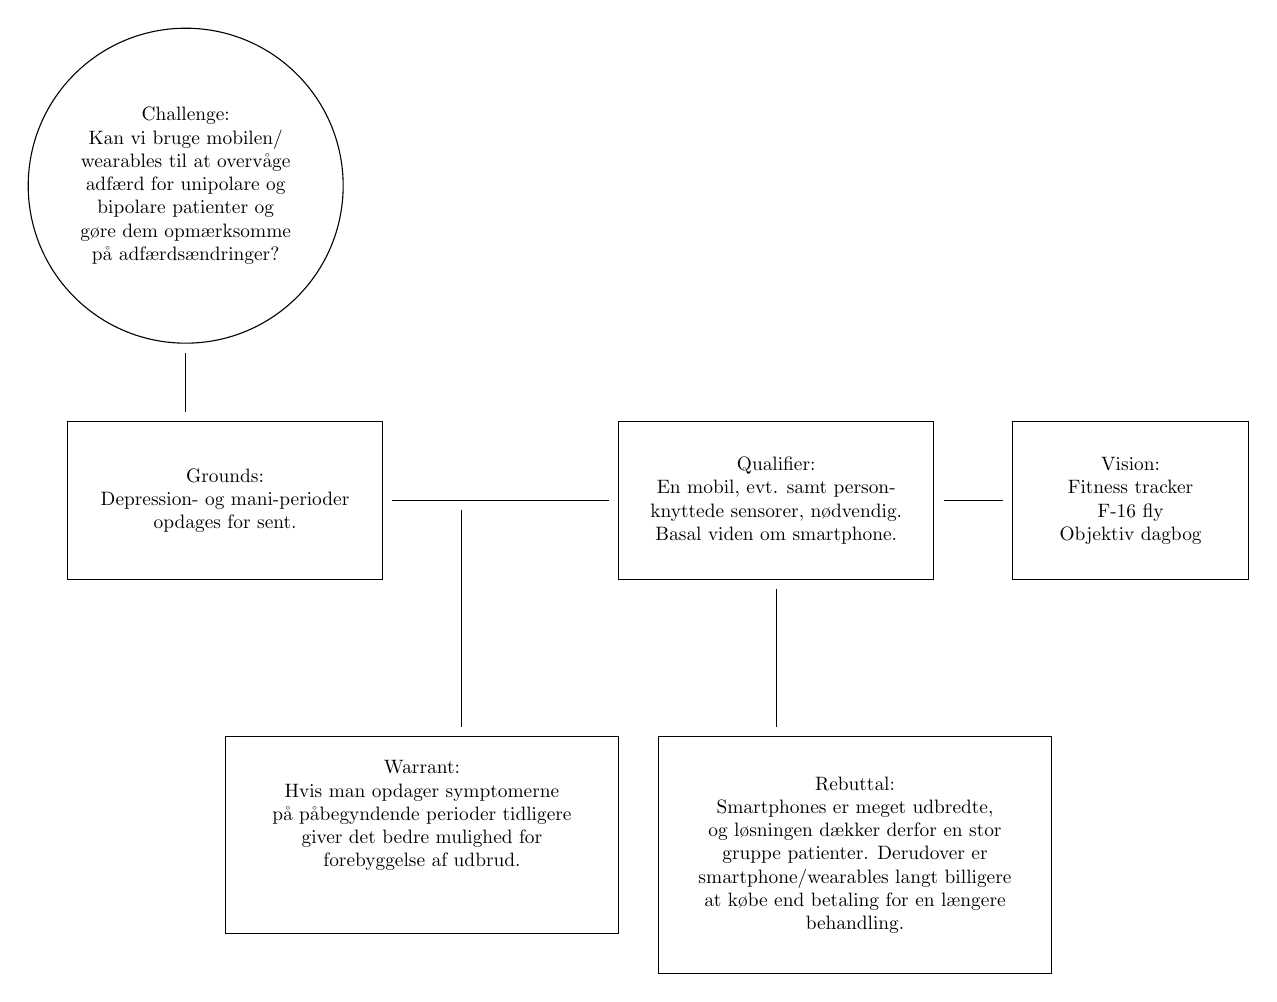
\begin{tikzpicture}

\draw  (-14,7) rectangle (-10,5);
\draw  (-12,3) rectangle (-7,0.5);
\draw  (-6.5,3) rectangle (-1.5,0);
\draw  (-7,7) rectangle (-3,5);
\draw  (-2,7) rectangle (1,5);

\node (v1) at (-10,6) {};

\node (v2) at (-7,6) {};
\draw  (v1) edge (v2);


\node (v3) at (-9,6) {};
\node (v4) at (-9,3) {};
\draw  (v3) edge (v4);
\node (v5) at (-5,3) {};
\node (v6) at (-5,5) {};
\draw  (v5) edge (v6);
\node (v7) at (-3,6) {};
\node (v8) at (-2,6) {};
\draw  (v7) edge (v8);



\draw  (-12.5,10) ellipse (2 and 2);
\node[align=center,scale=0.7] at (-12.5,10) {Challenge: \\Kan vi bruge mobilen/\\wearables  til at overvåge \\ adfærd for unipolare og \\ bipolare patienter og \\gøre dem opmærksomme\\ på adfærdsændringer?};

\node[align=center,scale=0.7] at (-12,6) {Grounds:\\Depression- og mani-perioder\\ opdages for sent.};
\node[align=center,scale=0.7] at (-9.5,2) {Warrant: \\Hvis man opdager symptomerne\\ på påbegyndende perioder tidligere\\ giver det bedre mulighed for\\ forebyggelse af udbrud.};

\node[align=center,scale=0.7] at (-5,6) {Qualifier:\\En mobil, evt. samt person-\\knyttede sensorer, nødvendig.\\ Basal viden om smartphone.};
\node[align=center,scale=0.7] at (-4,1.5) {Rebuttal:\\Smartphones er meget udbredte,\\ og løsningen dækker derfor en stor\\ gruppe patienter. Derudover er\\ smartphone/wearables langt billigere\\ at købe end betaling for en længere\\ behandling.};
\node[align=center,scale=0.7] at (-0.5,6) {Vision:\\Fitness tracker\\F-16 fly\\Objektiv dagbog};

\node (v10) at (-12.5,8) {};
\node (v9) at (-12.5,7) {};
\draw  (v9) edge (v10);
\end{tikzpicture}
    
    }
	\caption{Vision mønstret for projektet.}
	\label{fig:visionpattern}
\end{figure}

\subsubsection{Prospects research}
Problemer en projektgruppe støder på, der kræver undersøgelse for at opnå ny viden, er et \textit{Prospect}.
Det er så op til projektgruppen at vælge, om de vil investere i de \textit{Prospects} de har. \cite[nederst på side 104]{art:essence}

Dette er en liste over de \textit{Prospects} der er fundet ift. dette projekt, præsenteret som spørgsmål:
\begin{itemize}
	\item Hvordan kan det afgøres hvilken kontekst en mobiltelefon er i? fx i jakkelommen, på natbordet eller på patienten.
	\item Hvordan kan pladsforbruget af systemet mindskes?
	\item Hvordan kan strømforbruget af systemet mindskes?
\end{itemize}
Ingen af disse \textit{Prospects} blev valgt at blive udført af projektgruppen. % A representation of your Project Vision and (if relevant) Prospect Research (see Essence-book Chapter 15).
\section{Kriterier}
Her vil de vigtigste kriterier, som skal opfyldes for at kunne kalde projektet en succes, blive præsenteret.
Disse kriterier dækker over to overordnede områder: i forhold til bruger, og i forhold til platformen i sig selv.

\subsection{Bruger}

\subsubsection{Sikkerhed}
Da systemet, afhængigt af valgte moduler, kan indeholde person-følsomme data er det vigtigt at denne data er opbevaret sikkert og ikke kan tilgås af udefrakommende processer der ønsker at bruge den data til andet end helbredsestimering.
\bruno{Moduler er ikke nævnt her endnu.}

\subsubsection{Stabilitet}
For at sikre der ikke opstår for mange huller i den indsamlede data, skal systemet køre stabilt, så der kontinuert kan indsamles data.
Hvis der opstår for mange huller, kan dette give et ufuldstændigt billede af patientens sindstilstand, som måske kan fejl-fortolkes.

\subsubsection{Præcision}
Ligesom ved huller i indsamlingen af data over tid, er det lige så vigtigt at den data der kommer ind er præcis.
Dette er især også gældende for den måde som analyse-moduler fortolker den rå data, da fejl i analyser vil kunne give et forkert billede af patientens sindstilstand.

\subsection{Platform}

\subsubsection{Fleksibilitet}
Det skal være nemt at modificere selve platformen (ikke kun tilføjelse af nye moduler), da det stadig er et usikkert område der opereres indenfor.
Disse usikkerheder gælder både problemområde og den platform der implementeres på (Android).

\subsubsection{Mulighed for udvidelse}
Det skal være muligt at udvide platformen, uden at modificere platformens kodebase.
Dette skal gøres med moduler.
Det skal gøres på sådan en måde at personer der ikke er en del af systemet, kan lave og tilføje egne moduler.
Dette giver naturligvis yderligere overvejelser ift. sikkerhed.

\subsection{Evaluering af kriterier}
\mikael{Hvordan skal vi evaluere på de kriterier? Hvad kunne være godt at gøre? Hvad har vi egentlig tænkt os at gøre?}
\bruno{Igen +1 til Mikael - damn it..}
 % Key criteria for evaluations in your project plus one or more examples of evaluations  (see Essence-book Chapter 16).
\section{Vision Scenarios}
Hele dette afsnit er bygger på \citet[Sektion 17.1]{art:essence}, hvor der foreslås en teknik kaldet \textit{vision scenarios} til at nærmere bestemme fokus for et projekt.
For at styre dette projekt i den rigtige retning er der blevet lavet vision scenarios som hjælper med dette.
Til at lave vision scenarios er det nødvendigt at tildele roller til de forskellige personer der er med i projektet.
Rollerne der skal udleves er Child \citep[Kapitel 18]{art:essence}, Challenger \citep[Kapitel 19]{art:essence}, Responder \citep[Kapitel 20]{art:essence} og Anchor \citep[Kapitel 21]{art:essence}.

\subsection{Bestemmelse af retning}
For at hjælpe med at bestemme retning for projektet, hvor der var flere interessante bud, opsættes \textit{vision scenarios}.
Her sættes flere modsætninger overfor hinanden, hvor hver modsætningspar kan føre projektet i to forskellige retninger.
I vores tilfælde fandt vi seks forskellige modsætninger vi syntes kunne være interessante at kigge på:
\begin{itemize}
	\item Én Lidelse kontra Flere lidelser
	\item Personligt kontra Delt med læge
	\item Udregning i skyen kontra Lokal udregning
	\item Opbevaring i skyen kontra Lokal opbevaring
	\item Bruger input kontra Sensor input
	\item Interventioner kontra Patient empowerment
\end{itemize}

Ud af disse seks modsætningspar blev udvalgt de 2 vurderet mest relevante, hvilket blev gjort på demokratisk vis.
Dette førte til en 2-dimensioneal sammenligning, hvor på den ene akse er der opsat \textit{Bruger input} gående mod \textit{Sensor input} og på den anden akse \textit{Interventioner} gående mod \textit{Patient empowerment}.
Derefter anskues alle 4 kombinationer af begreber med de 4 forskellige roller.

\newcommand{\coord}[8]{
\begin{center}
\resizebox{0.6\columnwidth}{!}{
		\begin{tikzpicture}
			[
			    scale=5,
				axis/.style={very thick, <->, >=stealth'},
				important line/.style={thick},
				dashed line/.style={dashed, thin},
				pile/.style={thick, ->, >=stealth', shorten <=2pt, shorten
				>=2pt},
				every node/.style={color=black}
				]
				\tikzstyle{every node}=[font=\small]
				\draw[axis] (-1,0) node(xline)[below]{#1}  -- (1,0) node(xline)[below]{#2};
				\draw[axis] (0,-1) node(yline)[right]{#4} -- (0,1) node(yline)[left]{#3};
				\node[draw=none,align=center,text width=3cm] at (-0.5,0.5){#5};
				\node[draw=none,align=center,text width=3cm] at (0.5,0.5){#6};
				\node[draw=none,align=center,text width=3cm] at (0.5,-0.5){#7};
				\node[draw=none,align=center,text width=3cm] at (-0.5,-0.5){#8};
		\end{tikzpicture}
		}
\end{center}
}


\subsection{Child}
Dette er den eneste rolle alle i projektet kan have på vilkårlige tidspunkter.
Det er også denne rolle der sørger for at der kommer kreative idéer og er helt central for hvordan idéer bliver lavet i samarbejde mellem udviklere og kunder.

\coord
  {Bruger Input}
  {Sensor Input}
  {Interventioner}
  {Patient Empowerment}
  {Brug bruger input til at opdage påbegyndende forværring i tilstand og oplys patienten om dette.}
  {Brug objektive datakilder til at opdage påbegyndende forværring i tilstand og oplys patienten om dette.}
  {Brug objektive datakilder til at informere patienten om sin nuværende tilstand.}
  {Brug bruger input til at informere patient om sin nuværende tilstand.}

\subsection{Challenger}
Det er den der snakker på vegne af \textit{stakeholders}.
Det er også ud fra denne rolle der gives opgaver, prioriteres opgaver og accepteres løsninger.
Derudover skal dem som har rollen være inspirerende i den forstand at de skal kunne få udviklere til at se flere mulige løsninger. 
Challenger bruges på denne måde til at sørge for at den løsning der vælges er den rigtige løsning, samt om det er den bedste løsning der kan blive lavet.

\coord
  {Bruger Input}
  {Sensor Input}
  {Interventioner}
  {Patient Empowerment}
  {Ud fra bruger input foreslås lystbetonede aktiviteter.}
  {Ud fra sensor input registeres ændring i adfærd til at foreslå lystbetonede aktiviteter.}
  {Visualisere sensor input så brugeren kan blive opmærksom på sine ændringer i adfærd.}
  {Visualisere bruger input så brugeren kan blive opmærksom på sine ændringer i stemningsleje.}

\subsection{Responder}
Responders opgaver består i at lave mulige løsninger om til færdige løsninger og at løse de forskellige opgaver der bliver givet.
Denne rolle består af udviklerne og det er derfor denne rolle der står for prototypes og alle de tekniske løsninger.
Responder rollen bruges til at se om man har udnyttet det fulde potentiale af projektet.
Her er der tale om man bruger de rigtige komponenter, men også om man bruger disse komponenter så meget som man overhovedet kan. 

\coord
  {Bruger Input}
  {Sensor Input}
  {Interventioner}
  {Patient Empowerment}
  {Tilpasset dagbog baseret på tidligere dagbogsindlæg.
    Struktureret så data kan analyseres og sammenlignes og derudfra foretage interventioner.}
  {Brug sensor data til at foreslå interventioner til brugeren baseret på trends, fx. gang, søvn eller social aktivitet.}
  {Visualisere sensor data så patienten kan vurdere sin tilstand.}
  {Elektronisk dagbog med løs tekst.}

\subsection{Anchor}
Anchor er den der skal beskytte udviklerne fra at blive forstyrret og glemme hvad fokus er.
Dernæst er det også denne rolle der sørger for at planlægge specielle events, såsom sprint planning.
Anchors rolle er at sørge for at alle stakeholders er tilfredse med det der bliver udviklet.
Derudover er det også deres opgave at beskrive de fordele og ulemper der er ved de forskellige idéer, visioner, prototyper og strategier.

\coord
  {Bruger Input}
  {Sensor Input}
  {Interventioner}
  {Patient Empowerment}
  {Hvordan kan det afgøres om man skal foretage interventioner.
    Hvordan kan dagbogindslag sammenlignes.
    Hvordan vælges hvilken intervention.}
  {Hvordan kan det afgøres om der skal foretages en intervention.
    Hvordan identificere man treds og ændring i adfærd.
    Hvordan vælges hvilken intervention.}
  {Hvordan kan man visualisere meget data.
    Hvordan kan data aggregeres.}
  {Hvordan får brugeren overblik over sin dagbog.}
 % Characterization of your project using Vision Scenarios  (see Essence-book Part 4):
\section{Example of Idea Maturation}

Der er mange ændringer, vi snakker om disse:

Evaluation

Stakeholders

Features

\todo[inline]{skriv ting}

\begin{figure}
	\includegraphics[scale = 0.65,trim = 1cm 3cm 6cm 2cm, angle = 90, clip]{tidligfisk.pdf}
	\caption{En konfigurationstabel på et tidligt stadie af udviklingen}
	\label{tab:tidligKonfigurationsTabel}
\end{figure} % Give an example of idea maturation
\section{Theoretical Evaluation}

\subsection{Community}
% Udvikling sker ikke i vakum
% noget om social interaktion og ny viden
Som nævnt i \citet[Kapitel 2]{book:softwareinnovation} foregår software-udvikling sjældent i et vakuum.
Den meste udvikling foregår som del af en social proces, dette er især gældende for innovativ udvikling.
Ved at arbejde indenfor communities, enten åbne eller lukkede, er der større mulighed for at lufte og udforske idéer og derved få afprøvet og bekræftet disse, samt mulighed for videre udvikling med andre interesserede.
I disse communities er det også muligt at finde eksperter indenfor andre områder, så der også på denne måde kan deles allerede eksisterende viden, som yderlige kan assistere ved tilblivelsen af nye idéer.

Disse ting gør sig også gældende for vores projekt, hvor vi er interesseret i at både dele og opnå viden, for at kunne levere det bedst mulige produkt, altså hvor vi bedst muligt kan hjælpe personer med psykiske lidelser.
Dette er viden fra andre udviklere, fagfolk og potentielle brugere.

\subsubsection{En åben platform}
% Åben/fleksibel struktur/arkitektur
% Mulighed for udvikling af nye moduler og deling af disse
% Udviklere vha kode, fagfolk vha grafisk værktøj. lissom Mindstorms
PsyLog platformen er udviklet som en fleksibel struktur, der tillader uafhængig udvikling af nye moduler.
Strukturen anvender moduler som byggesten ved, for det første, at lade patienten bestemme kombinationen af moduler på hans mobiltelefon og for det andet ved at tillade at alle kan udvikle nye moduler.

Herved kan systemet betragtes som et fælles system som alle har mulighed for at bidrage til.
Platformen og de moduler der er udviklet hertil er tilgængelige via \href{http://github.com}{github.com}.
På samme måde kan moduler udviklet i fremtiden deles via en open source platform.
Med denne tilgang kan man forestille sig en situation hvor innovation kan ske parallelt på flere uafhængige lokationer.
Altså kan man forestille sig en situation hvor man fx ved psykiatrien i Aalborg (eventuelt i forbindelse med semesterprojekter ved Aalborg universitet) udvikler moduler med særligt fokus på social aktivitet, mens man i København fokuserer på søvnbesvær.
På den måde kan udviklingen af nye og forbedringen af eksisterende moduler ske de steder hvor fokus på dem er særligt store.
Dermed kan den faglige ekspertise fra psykiatere og psykologer inddrages til udvikling af moduler der særligt relaterer sig til deres fokusområde.

\subsubsection{Udviklingsmetoder}
I kraft af at udviklingen af PsyLog platformen er sket i forbindelse med et semesterprojekt på en software uddannelse er kravene for udviklingen af nye moduler tilsvarende tekniske.
For at løse denne problemstilling kunne en løsning, som den LEGO har anvendt til deres Mindstorms produkter, anvendes.
Her programmeres en robot ved hjælp af et grafisk \textit{''programmeringssprog''} for derved at gøre udviklingen mere tilgængelig.

For PsyLog kunne der anvendes en lignende tilgang hvor fagfolk (psykiatere og psykologer) kombinerer eksisterende moduler og et mængde simple operationer for derved at skabe nyt indhold.
\subsection{Proces}
% the steps, tools and practices that you used to arrive at your results
For at opnå vores resultat, har vi brugt forskellige redskaber og praksiser.
I dette afsnit detaljerer og evaluerer vi dem, baseret på \citet{book:softwareinnovation}.
\subsection{Tools}
Gennem vores arbejde blev der anvendt en række redskaber, som udviklerne havde erfaring med på forhånd.
Dette svarer fint til beskrivelsen i \citet[Kapitel 7]{} hvor der lægges op til at udviklerne har en værktøjskasse med en række redskaber, der kan benyttes.

Et redskab der blev benyttet er prototyping.
Det blev brugt til at komme med low-fidelity bud på løsninger, eksempelvis var det meget nyttigt til at komme med foreslag til vores indstillingsmenu.

Brainstorming blev benyttet, bl.a. var det nyttigt til at få en række idéer til dataindsamlings- og analyse-moduler.

\subsection{Improvisering}
Improvisering er en stor del af software innovation som \citet[side 56]{book:softwareinnovation} siger: \textit{Improvisation and bricolage flesh out the skeleton, whatever the underlying process. Developing technically exploratory software involves manoeuvring in uncharted waters, where development platforms are uncertain and untried, so it is unlikely that generic process models or formal development methods can provide enough support for the developer.}
Derfor har det selvfølgelig også været en stor del af vores proces, og denne improvisering har taget forskellige former.
Som \citet[side 56]{book:softwareinnovation} siger: \textit{In a development situation, improvisation often takes the form "let's try this...:" a customer meeting, a programming technique, a diagramming technique, a different hardware component.}
Af disse former har vi mødt med interesserede personer og patienter med psykiske lidelse for at få deres perspektiv og deres idéer om platformen og hvad der kan gøres med de data kilder der er tilgængelige. 
Ydermere har vi brugt brainstorming, idet vi så på de forskellige sensorer og kom med idéer om hvad de kunne bruges til for at få kontaktpersonernes holdninger om dette.
På samme tid har vi også brugt diagram teknikker, til at afklare hvordan en arkitektur passende til de krav vi fik gennem kontaktpersoner og patienter skulle se ud.
Teknikker er blevet brugt til at lave flere versioner af arkitekturen og af disse er der blevet foretaget et valg.
\subsection{Software team dynamik}
Om et software team er innovativt afhænger af en mængde faktorer som teamet sjældent har kontrol over.
Disse faktorer varierer fra omgivelserne de sidder i, til de krav der bliver stillet fra deres overordnede.
Et udvalg af disse faktorer vil i dette blive beskrevet (taget fra \citet[s.~81-82]{book:softwareinnovation}), hvorefter vi vil vurdere deres indflydelse på vores projekt.

\begin{description}[style=nextline]
	\item[Tidspres] Når et team arbejder under tidspres forhindrer det at teamet bruger tid på refleksion, hvilket udelukker at der bruges tid på at udforske og eksperimentere med mulige løsninger.
	\item[Stress] Stress har både fysiologiske og psykologiske effekt på produktiviteten. Når et team er stresset forværres kommunikationen internt hvilket har en negativ effekt på produktet.
	\item[Ressource mangel] Mangel på ressourcer tvinger teamet til de vante arbejdsgange, i stedet for eksperimenterende tilgange til problemer.
	\item[Strengt definerede arbejdsgange] Hvis teamet er tvunget til et sæt af prædefinerede arbejdsgange fra deres overordnede besværliggør det refleksion.
	\item[Bureaukrati] Overdokumentation af teamets arbejde tvinger holdet til at følge de definerede processer 
	\item[Rutinearbejde] For meget rutinearbejde får teamets medlemmer til ikke at se opgaverne i et alternativt perspektiv.
	\item[Dårlig projektstyring] Autoritære projektstyringsstile har en negativ indflydelse på innovative karakteristikker som dialog.
\end{description}

I det følgende vil det blive beskrevet 

\paragraph{Semester}
Da vi er dikterede af studieordningens indhold er der nogle forhold som vi ikke selv er herre over.
For det første løber semestret over en prædefineret periode hvilket introducerer et \textbf{tidspres}.
Studieordningen kræver også at arbejdet bliver dokumenteret i en rapport hvilket er en blanding af \textbf{bureaukrati} og \textbf{strengt definerede arbejdsgange}.

\paragraph{Vejleder}
En barriere der ikke har været i projektet er \textbf{ressource mangel}, da vores vejleder fra starten har bidraget til projektet både med indsigt og med ressourcer som smartphone og smartwatch.

\paragraph{Teamet}
Teamet har i til dels været tilbøjelig til \textbf{rutinearbejde} i forhold til strukturen i projektet.
Tasks defineres, kodes og dokumenteres uden videre eftertanke om, hvorvidt vi er på vej i den rigtige retning.
\textbf{Dårlig projektstyring} er i kilden defineret ud fra autoritære projektstyringsstile.
I vores projekt har det omvendte været problemet, der har ikke været én projektleder, men i stedet har vi alle haft en del af lederrollen.
Dette har betydet at ledelsen har været løs og uden retning. % Theoretical evaluation. Compare your work with some of the theories that are referred to in the course literature. The evaluation should not be value judgment-based, but should seek to relate your work to the theories and principles that the course draws from. You might like to focus on 

\bibliographystyle{unsrtnat}
\bibliography{bib}
\label{bib:mybiblio}

\appendix
%\chapter{Dogmeregler}\label{app:dogmeregler}
\begin{enumerate}
	\item De bedste logdata indsamlinger er funderet i psykologisk/psykiatrisk teori.
	\item Dataindsamlingen skal foregå med så lav en pris som muligt. Dvs enhver patient interaktion med systemet er en omkostning.
	\item Systemet skal have en ideografisk menneskesyn.
	\item Systemet skal understøtte intervention, altså eksperimenter.
	\item Systemet skal støtte patient empowerment og patienten skal selv kunne se egen data og statistikker i meningsfyldte dashboards og datavisualiseringer.
	\item Dataindsamlingen skal foregå med så lav en pris som muligt. Dvs enhver patient interaktion med systemet er en omkostning.
	\item Når patienten skal interagere med systemet skal det forståes og opleves af patienten som en del af en behandling. Ikke som en del teknisk indstilling af systemet.
	\item Idet logdataene er "det rene empiri" skal systemet selv kunne eliminere eller gøre opmærksom på anormalier.
	\item For at sikre validiteten af dataene skal dataindsamlingen ikke kun være et sæt logdata, men flere, som gør det muligt få en høj validitet af resultaterne samt at eliminere fejlagtige datasæt.
	\item Systemet skal ikke være et blackbox system, men et whitebox.
\end{enumerate}

\end{document}
